\subsection{Gradient Descent}
\noindent
Remember that if we have a multidimensional function, taking a step in the direction of the gradient results in the maximum possible increase of the function, and taking a step in the opposite direction of the gradient results in the maximum possible decrease of the function.
Gradient descent is a method to find minima of functions.\\

\noindent
Let's say we're trying to minimize $J(\vec{x})$ with gradient descent. Here are the steps we would take:
\begin{enumerate}
	\item Pick (or guess) a starting point $\vec{x_0}$ and a learning rate (step size) $\delta$.
	\item $\overrightarrow{x_{n+1}} = \overrightarrow{x_n} - \delta J(\overrightarrow{x_n})$
	\item Repeat step 2 until some stopping criteria is met, like $\norm{\delta \nabla J(\overrightarrow{x_n}) - \delta \nabla J(\overrightarrow{x_{n+1}})} < \epsilon$.
\end{enumerate}

\begin{figure}[H]
	\centering
	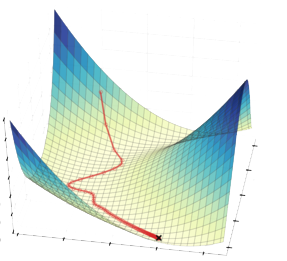
\includegraphics[width=0.5\textwidth]{./differentialMultivariableCalculus/gradient_descent.png}
	\caption{Path of several iterations of gradient descent}
\end{figure}

\noindent
This method will lead you arbitrarily close to a local minimum, but does not guarantee finding the global minimum.
More advanced versions of gradient descent exists that try to help with this, like giving the point ``momentum'' to be able to move out of local mins.
This method also has a trade off between speed and accuracy.
Although increasing $\delta$ means fewer iterations of gradient descent are needed to narrow in on a local minimum, one is more likely to be stuck in a local min than if they had used a smaller $\delta$.\\

\noindent
In the real world, the function you are trying to minimize will likely not be well defined enough to take its partial derivatives to find the gradient, so they too are approximated by doing something like
\begin{equation*}
	J_{k} = \frac{J(k+.0001, \ldots) - J(k, \ldots)}{.0001}.
\end{equation*}